\section*{Figure captions:}
\begin{figure}[H]
\begin{center}
\scalebox{0.85}{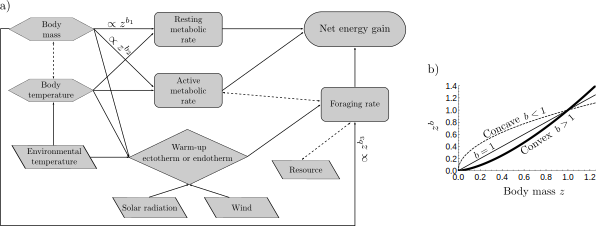
\includegraphics{fig1}}
\caption{
	Panel a) shows the link between the components of the model.
	Unidirectional solid lines mean the first component affects the second component it points at.
	Bidirectional dashed lines represent a correlation or an indirect link between the two components.
	Panel b) visualizes the concavity ($b_3  = 1.25 > 1$) and convexity ($b_3 = 0.5 > 1$) of the power law relationship.
}
\label{fig1}
\end{center}
\end{figure}
%\vspace{-1.5cm} % E: consider \vfill
%\newpage
%
\begin{figure}[H]
\begin{center}
\scalebox{0.90}{\includegraphics{fig2}}
\caption{
	Different scenarios where net energy gain peaks at intermediate body size as funtion of resource quantity (a, b), resource quality (c, d), and temperature (e, f, g).
	%
	Exogenous parameters:
	For a) and b), abundant resource $R = 500$ (an individual can collect at most 50 times its body mass), scrace resource $R= 10$, resource quality $\rho = 12$, $T_e = 15$.
	For c) and d), high quality $\rho = 24$, low quality $\rho = 12$, total foraging time $\tau_f = 45 \rm{min}$, $T_e = 15$.
	For e)$T_e = 15$, for f) $T_e = 24.5$, $R = 500$, $\rho = 12$, and for g) $T_e = 17$
	Endogenous parameters:
	For a), b), c), d), and g) $b_2 = 0.75, a_2 = 20 a_1$.
	For e) and f) we assumed a high active metabolic rate $a_2 = 30 a_1, b_2  = 1.25$.
	Fixed parameter values: $b_1 = 0.75$.
	See \cref{table:table1} for units.
}
\label{fig2}
\end{center}
\end{figure}

\begin{figure}[H]
\begin{center}
\scalebox{0.85}{\includegraphics{fig3}}
\caption{
	Lowest temperature required for the completion of warm-up as a function of body mass.
	a)  low value for conductance (0.1 $\times$ the default value).
	b) default value for conductance, wind speed  = 0.1m/s.
	c)  $a_w = 1.25$.
	Fixed parameter values: default conductance $K_1 = 0.05 \, c_p, r_3 = 0.5$.
	Remaining parameters are in \cref{table:table1}.
	The individual is given a maximum of 6 hours to complete warm-up.
	To focus on the effect of solar radiation, daily temperature is constant.
	Solar radiation increases linearly from 0 to 0.25 of the maximum value $S_0$ during a period of 6 hours.
	See \cref{table:table1} for units.
}
\label{fig3}
\end{center}
\end{figure}
%
\begin{figure}[H]
\begin{center}
\scalebox{0.85}{
\includegraphics{fig4}}
\caption{
	Panel a) shows the duration of warm-up as a function of the timing of warm-up and body size for ecotherm (similar results for endotherms).
	Panel b) shows the duration of warm-up as a function of the conductance for endotherms. Body size $z = 1$ , $a_w = 1.25$
	Solar radiation is equivalent to what would happen at 30 degree latitude during equinox.
	Environmental temperature $ T_e = 15$.
	Default value $K_1$ in a) and $K_2$ a) and b).
	See \cref{table:table1} for units.
}
\label{fig4}
\end{center}
\end{figure}
\vspace{-0.8cm}
%\newpage
%%
\begin{figure}%[H]
\begin{center}
\scalebox{0.85}{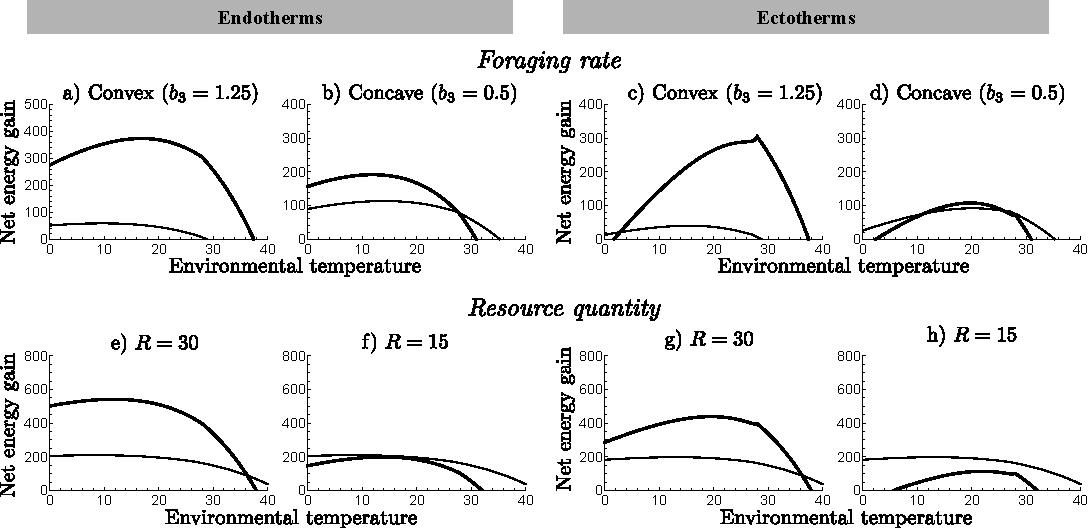
\includegraphics{fig5}}
\caption{
	Overlap of the thermal performance curves (or net energy gain) between body sizes as function of: the timing of warm-up (a,b), the exponent of the foraging rate (c,d), and the quantity of resource available (e, f).
	Exogenous parameters:
	$\rho = 30, R = 30 \rm{g}$ expect for f) $R = 15 \rm{g}$.
	%
	Endogenous parameters:
	For c) and d) convex ($b_3 = 1.25$) concave ($b_3 = 0.5$).
	For e) and d) $b_3 = b_2 = b_1 = 0.75$.
	For a), b), c), and d) large $z = 2 \rm{g}$, small $z = 0.5 \rm{g}$.
	For e) and f) large $z = 2 \rm{g}$, small $z = 0.1 \rm{g}$.
	%
	Other parameters:
	Foraging time $\tau_f = 1 \rm{hour}$ and $a_2 = 10 a_1$, wind $u = 1 \rm{m.s^{-1}}$.
	See \cref{table:table1} for units.
}
\label{fig5}
\end{center}
\end{figure}

%
% \section*{Figure captions:}
% \begin{figure}[H]
% \begin{center}
% \scalebox{0.85}{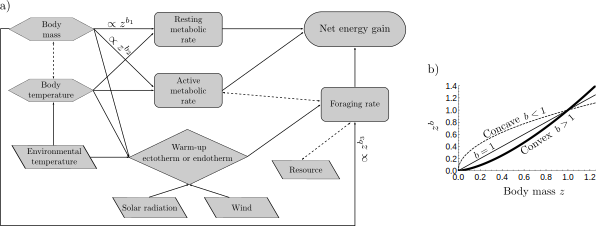
\includegraphics{fig1}}
% \caption{
% 	Panel a) shows the link between the components of the model.
% 	Unidirectional solid lines mean the first component affects the second component it points at.
% 	Bidirectional dashed lines represent a correlation or an indirect link between the two components.
% 	Panel b) visualizes the concavity ($b_3  = 1.25 > 1$) and convexity ($b_3 = 0.5 > 1$) of the power law relationship.
% }
% \label{fig1}
% \end{center}
% \end{figure}
% %\vspace{-1.5cm} % E: consider \vfill
% %\newpage
% %
% \begin{figure}[H]
% \begin{center}
% \scalebox{0.90}{\includegraphics{fig2}}
% \caption{
% 	Different scenarios where net energy gain peaks at intermediate body size as funtion of resource quantity (a, b), resource quality (c, d), and temperature (e, f, g).
% 	%
% 	Exogenous parameters:
% 	For a) and b), abundant resource $R = 500 \rm{g}$ (an individual can collect at most 50 times its body mass), scrace resource $R= 10 \rm{g}$, resource quality $\rho = 12 \rm{J.g^{-1}}$, $T_e = = 15 ^{\circ} \rm{C}.$
% 	For c) and d), high quality $\rho = 24 \rm{J.g^{-1}}$, low quality $\rho = 12 \rm{J.g^{-1}}$, total foraging time $\tau_f = 45 \rm{min}$, $T_e = = 15 ^{\circ} \rm{C}$.
% 	For e)$T_e = 15 ^{\circ} \rm{C}$, for f) $T_e = 24.5 ^{\circ} \rm{C}$, $R = 500 \rm{g}$, $\rho = 12 \rm{J.g^{-1}}$, and for g) $T_e = 17 ^{\circ} \rm{C}$
% 	Endogenous parameters:
% 	For a), b), c), d), and g) $b_2 = 0.75, a_2 = 20 a_1$.
% 	For e) and f) we assumed a high active metabolic rate $a_2 = 30 a_1, b_2  = 1.25$.
% 	Fixed parameter values: $b_1 = 0.75$.
% }
% \label{fig2}
% \end{center}
% \end{figure}
% %\vspace{-1.5cm}
% %\newpage
% %
% % \begin{figure}[H]
% % \begin{center}
% % \scalebox{0.85}{\includegraphics{fig3}}
% % \caption{
% % 	 Daily net energy gain  $E_n$ as a function of body mass $z$ without warm-up, and foraging time limited to 0.5 hour.
% % 	a) Daily net energy gain  $E_n$ as a function of body mass $z$ for different value of foraging exponent $b_3 = 0.5, 0.8, 1.25$, dashed, thin, thick lines respectively  at $T_e  = 15 ^{\circ} \rm{C}$.
% % 	b) $E_n$ is maximized at an intermediate value of $z$  when shaded regions and resource quality $\rho$ intersect (i.e., \cref{eq:C1} is satisfied).
% % 	Warm ($35^{\circ} \rm{C}$) and cold (15$^{\circ} \rm{C}$) environmental temperatures are denoted by red and cyan, respectively.
% % 	The upper (lower) limit of the shaded region is $\widetilde{dE_n}$ ($\widetilde{E_n}$).
% % 	c) Various shapes of $E_n$ based on b).
% % 	In b) and c), $\rho = 13, 60, 100$ dashed, thin, and thick, respectively.
% % 	Fixed parameter values: $b_1 = b_2 = 0.75, a_2 = 5 a_1, $.
% % }
% % \label{fig3}
% % \end{center}
% % \end{figure}
% %\vspace{-1.5cm}
% %\newpage
% %
% \begin{figure}[H]
% \begin{center}
% \scalebox{0.85}{\includegraphics{fig3}}
% \caption{
% 	Lowest temperature required for the completion of warm-up as a function of body mass.
% 	a)  low value for conductance (0.1 $\times$ the default value).
% 	b) default value for conductance, wind speed  = 0.1m/s.
% 	c)  $a_w = 1.25$.
% 	Fixed parameter values: default conductance $K_1 = 0.05 \, c_p, r_3 = 0.5$.
% 	Remaining parameters are in \cref{table:table1}.
% 	The individual is given a maximum of 6 hours to complete warm-up.
% 	To focus on the effect of solar radiation, daily temperature is constant.
% 	Solar radiation increases linearly from 0 to 0.25 of the maximum value $S_0$ during a period of 6 hours.
% }% Add parameter values later
% \label{fig3}
% \end{center}
% \end{figure}
% %\vspace{-1.5cm}
% %\newpage
% %
% \begin{figure}[H]
% \begin{center}
% \scalebox{0.85}{
\includegraphics{fig4}}
% \caption{
% 	Panel a) shows the duration of warm-up as a function of the timing of warm-up and body size for ecotherm (similar results for endotherms).
% 	Panel b) shows the duration of warm-up as a function of the conductance for endotherms. Body size $z = 1$ , $a_w = 1.25$
% 	Solar radiation is equivalent to what would happen at 30 degree latitude during equinox.
% 	Environmental temperature $ T_e = 15^{\circ}\rm{C}$.
% 	Default value $K_1$ in a) and $K_2$ a) and b) .
% }% Add parameter values later
% \label{fig5}
% \end{center}
% \end{figure}
% \vspace{-0.8cm}
% %\newpage
% %%
% \begin{figure}%[H]
% \begin{center}
% \scalebox{0.85}{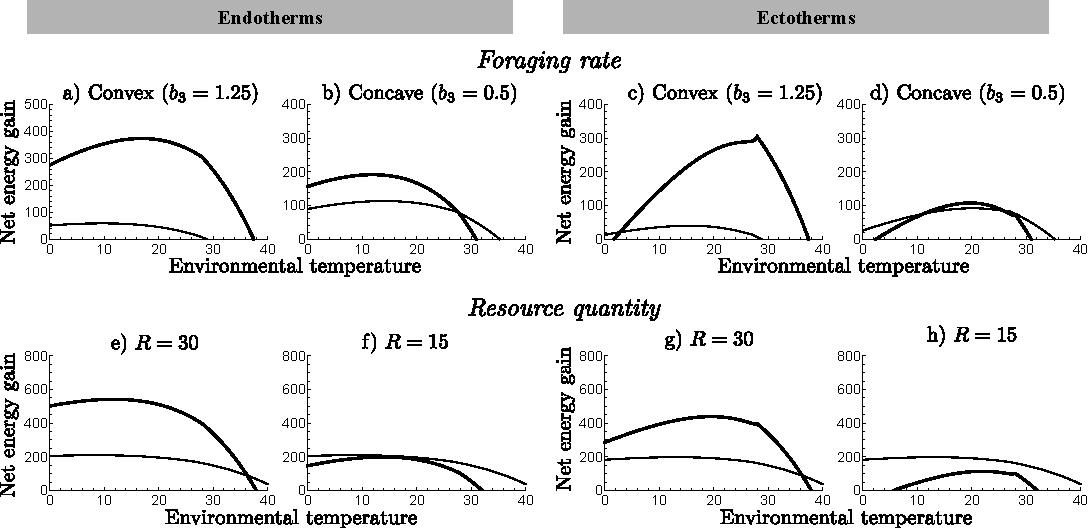
\includegraphics{fig5}}
% \caption{
% 	Overlap of the thermal performance curves (or net energy gain) between body sizes as function of: the timing of warm-up (a,b), the exponent of the foraging rate (c,d), and the quantity of resource available (e, f).
% 	Exogenous parameters:
% 	$\rho = 30, R = 30 \rm{g}$ expect for f) $R = 15 \rm{g}$.
% 	%
% 	Endogenous parameters:
% 	For c) and d) convex ($b_3 = 1.25$) concave ($b_3 = 0.5$).
% 	For e) and d) $b_3 = b_2 = b_1 = 0.75$.
% 	For a), b), c), and d) large $z = 2 \rm{g}$, small $z = 0.5 \rm{g}$.
% 	For e) and f) large $z = 2 \rm{g}$, small $z = 0.1 \rm{g}$.
% 	%
% 	Other parameters:
% 	Foraging time $\tau_f = 1 \rm{hour}$ and $a_2 = 10 a_1$, wind $u = 1 \rm{m.s^{-1}}$.
%
% }% Add non trivial units later
% \label{fig5}
% \end{center}
% \end{figure}
